%% figures/fig-runaway.tex -- Figure for Sec. 1.4.
%% Pulled into notes.tex with %% figures/fig-runaway.tex -- Figure for Sec. 1.4.
%% Pulled into notes.tex with %% figures/fig-runaway.tex -- Figure for Sec. 1.4.
%% Pulled into notes.tex with %% figures/fig-runaway.tex -- Figure for Sec. 1.4.
%% Pulled into notes.tex with \input{figures/fig-runaway}.
%% Needs pgfplots, loaded in the main preamble.
%%
%% Panel (a) plots a = C exp(t/tau_0) for three values of C. Panel (b) plots
%% the impulse response of Eq. (AL): a = 0 before the blow and
%% a = kappa exp(t/tau_0) after it, with kappa = -J/(m tau_0). The sign is the
%% point of the panel and is not a drawing choice -- integrating
%% m a - m tau_0 adot = J delta(t) across t = 0 gives a jump of -J/(m tau_0),
%% so the runaway is directed against the impulse.

\begin{figure}[htb]
\centering
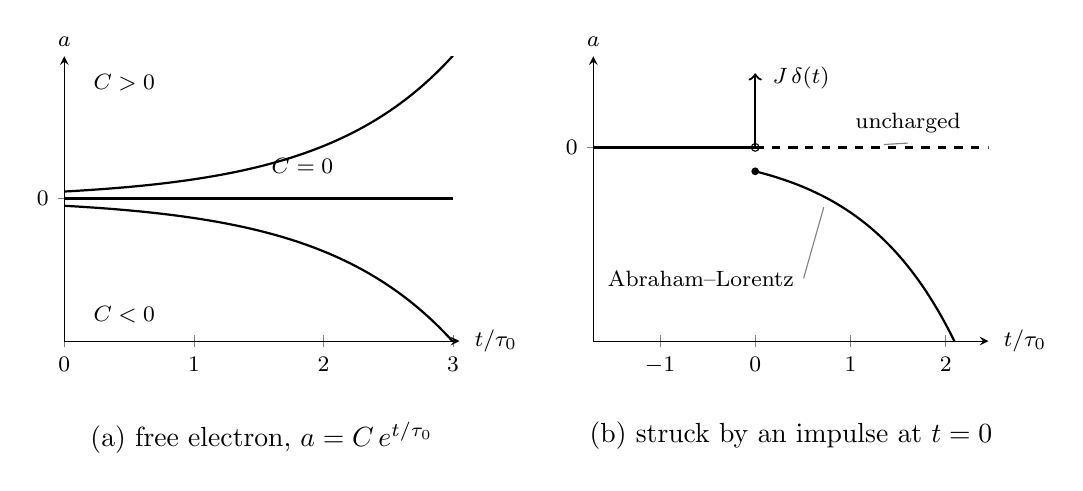
\begin{tikzpicture}

%% ---------------- panel (a): the free electron ----------------
\begin{axis}[
  name=free,
  width=6.6cm, height=5.2cm,
  xlabel={$t/\tau_0$}, ylabel={$a$},
  xmin=0, xmax=3.05, ymin=-3.2, ymax=3.2,
  axis lines=left,
  ytick={0}, yticklabels={$0$},
  xtick={0,1,2,3},
  every axis y label/.style={at={(ticklabel* cs:1.0)},anchor=south},
  every axis x label/.style={at={(ticklabel* cs:1.0)},anchor=west,
                             xshift=2pt},
  clip=true, samples=80, font=\footnotesize,
]
  \addplot[domain=0:3,thick] {0.16*exp(x)};
  \addplot[domain=0:3,thick] {-0.16*exp(x)};
  \addplot[domain=0:3,very thick] {0};
  \node[anchor=west,font=\footnotesize] at (axis cs:0.15,2.6)  {$C>0$};
  \node[anchor=west,font=\footnotesize] at (axis cs:0.15,-2.6) {$C<0$};
  \node[anchor=south east,font=\footnotesize] at (axis cs:2.15,0.35) {$C=0$};
\end{axis}
\node[anchor=north,align=center] at ([yshift=-9mm]free.south)
     {(a) free electron, $a=C\,e^{t/\tau_0}$};

%% ---------------- panel (b): struck by an impulse ----------------
\begin{axis}[
  name=imp,
  at={(free.east)}, anchor=west, xshift=1.7cm,
  width=6.6cm, height=5.2cm,
  xlabel={$t/\tau_0$}, ylabel={$a$},
  xmin=-1.7, xmax=2.45, ymin=-3.4, ymax=1.6,
  axis lines=left,
  ytick={0}, yticklabels={$0$},
  xtick={-1,0,1,2},
  every axis y label/.style={at={(ticklabel* cs:1.0)},anchor=south},
  every axis x label/.style={at={(ticklabel* cs:1.0)},anchor=west,
                             xshift=2pt},
  clip=true, samples=80, font=\footnotesize,
]
  %% before the blow: at rest
  \addplot[domain=-1.7:0,very thick] {0};
  %% uncharged particle: back to zero immediately
  \addplot[domain=0:2.45,very thick,dashed] {0};
  %% the impulse itself
  \draw[->,thick] (axis cs:0,0) -- (axis cs:0,1.3);
  \node[anchor=west,font=\footnotesize] at (axis cs:0.08,1.22) {$J\,\delta(t)$};
  %% Abraham-Lorentz: jumps the wrong way, then runs
  \addplot[domain=0:2.45,thick] {-0.42*exp(x)};
  \fill (axis cs:0,-0.42) circle (1.4pt);
  \draw (axis cs:0,0) circle (1.4pt);
  %% labels placed in the empty regions, with leaders
  \node[anchor=west,font=\footnotesize] (unch) at (axis cs:0.95,0.42)
       {uncharged};
  \draw[gray] (unch.south) -- (axis cs:1.35,0.05);
  \node[anchor=west,font=\footnotesize] (al) at (axis cs:-1.65,-2.3)
       {Abraham--Lorentz};
  \draw[gray] (al.east) -- (axis cs:0.72,-1.05);
\end{axis}
\node[anchor=north,align=center] at ([yshift=-9mm]imp.south)
     {(b) struck by an impulse at $t=0$};

\end{tikzpicture}
\caption{The two faces of the third-order term. \emph{(a)} A free electron
obeying Eq.~(\ref{eq:AL}) has $a = C\,e^{t/\tau_0}$. Every $C\ne0$ runs away;
the physical solution is the single value $C=0$, and nothing in the
initial-value problem selects it, since the equation is first order in $a$ and
admits any $a(0)$. \emph{(b)} An impulse delivered at $t=0$. An uncharged
particle takes the blow, jumps in velocity, and returns to zero acceleration:
the force is over and so is the acceleration. The electron does the opposite.
Its acceleration jumps to $\kappa = -J/m\tau_0$ and grows without bound long
after nothing is acting on it, and, since $\kappa$ carries the sign opposite to
$J$, it runs away against the blow that started it. The velocity, by contrast,
is continuous at $t=0$ here: it is the acceleration that jumps.
\label{fig:runaway}}
\end{figure}
.
%% Needs pgfplots, loaded in the main preamble.
%%
%% Panel (a) plots a = C exp(t/tau_0) for three values of C. Panel (b) plots
%% the impulse response of Eq. (AL): a = 0 before the blow and
%% a = kappa exp(t/tau_0) after it, with kappa = -J/(m tau_0). The sign is the
%% point of the panel and is not a drawing choice -- integrating
%% m a - m tau_0 adot = J delta(t) across t = 0 gives a jump of -J/(m tau_0),
%% so the runaway is directed against the impulse.

\begin{figure}[htb]
\centering
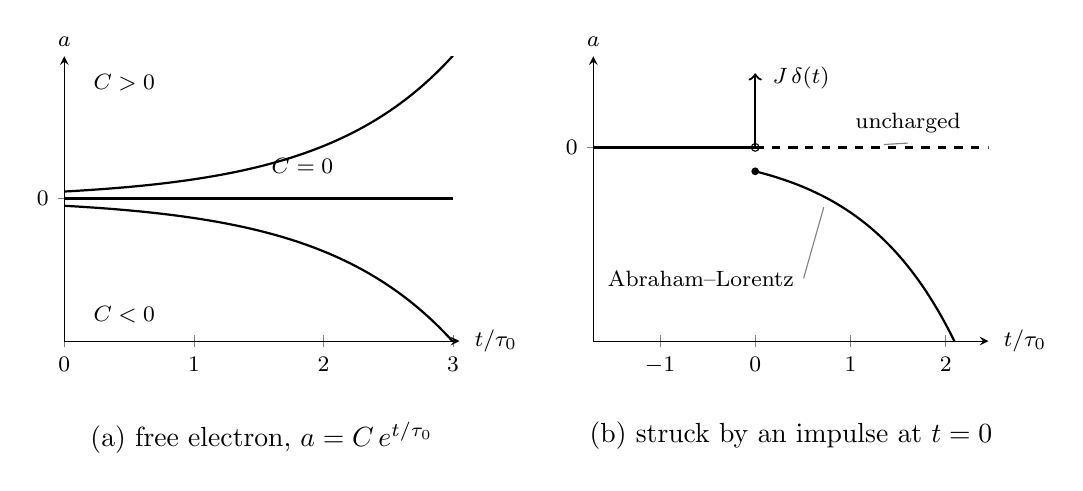
\begin{tikzpicture}

%% ---------------- panel (a): the free electron ----------------
\begin{axis}[
  name=free,
  width=6.6cm, height=5.2cm,
  xlabel={$t/\tau_0$}, ylabel={$a$},
  xmin=0, xmax=3.05, ymin=-3.2, ymax=3.2,
  axis lines=left,
  ytick={0}, yticklabels={$0$},
  xtick={0,1,2,3},
  every axis y label/.style={at={(ticklabel* cs:1.0)},anchor=south},
  every axis x label/.style={at={(ticklabel* cs:1.0)},anchor=west,
                             xshift=2pt},
  clip=true, samples=80, font=\footnotesize,
]
  \addplot[domain=0:3,thick] {0.16*exp(x)};
  \addplot[domain=0:3,thick] {-0.16*exp(x)};
  \addplot[domain=0:3,very thick] {0};
  \node[anchor=west,font=\footnotesize] at (axis cs:0.15,2.6)  {$C>0$};
  \node[anchor=west,font=\footnotesize] at (axis cs:0.15,-2.6) {$C<0$};
  \node[anchor=south east,font=\footnotesize] at (axis cs:2.15,0.35) {$C=0$};
\end{axis}
\node[anchor=north,align=center] at ([yshift=-9mm]free.south)
     {(a) free electron, $a=C\,e^{t/\tau_0}$};

%% ---------------- panel (b): struck by an impulse ----------------
\begin{axis}[
  name=imp,
  at={(free.east)}, anchor=west, xshift=1.7cm,
  width=6.6cm, height=5.2cm,
  xlabel={$t/\tau_0$}, ylabel={$a$},
  xmin=-1.7, xmax=2.45, ymin=-3.4, ymax=1.6,
  axis lines=left,
  ytick={0}, yticklabels={$0$},
  xtick={-1,0,1,2},
  every axis y label/.style={at={(ticklabel* cs:1.0)},anchor=south},
  every axis x label/.style={at={(ticklabel* cs:1.0)},anchor=west,
                             xshift=2pt},
  clip=true, samples=80, font=\footnotesize,
]
  %% before the blow: at rest
  \addplot[domain=-1.7:0,very thick] {0};
  %% uncharged particle: back to zero immediately
  \addplot[domain=0:2.45,very thick,dashed] {0};
  %% the impulse itself
  \draw[->,thick] (axis cs:0,0) -- (axis cs:0,1.3);
  \node[anchor=west,font=\footnotesize] at (axis cs:0.08,1.22) {$J\,\delta(t)$};
  %% Abraham-Lorentz: jumps the wrong way, then runs
  \addplot[domain=0:2.45,thick] {-0.42*exp(x)};
  \fill (axis cs:0,-0.42) circle (1.4pt);
  \draw (axis cs:0,0) circle (1.4pt);
  %% labels placed in the empty regions, with leaders
  \node[anchor=west,font=\footnotesize] (unch) at (axis cs:0.95,0.42)
       {uncharged};
  \draw[gray] (unch.south) -- (axis cs:1.35,0.05);
  \node[anchor=west,font=\footnotesize] (al) at (axis cs:-1.65,-2.3)
       {Abraham--Lorentz};
  \draw[gray] (al.east) -- (axis cs:0.72,-1.05);
\end{axis}
\node[anchor=north,align=center] at ([yshift=-9mm]imp.south)
     {(b) struck by an impulse at $t=0$};

\end{tikzpicture}
\caption{The two faces of the third-order term. \emph{(a)} A free electron
obeying Eq.~(\ref{eq:AL}) has $a = C\,e^{t/\tau_0}$. Every $C\ne0$ runs away;
the physical solution is the single value $C=0$, and nothing in the
initial-value problem selects it, since the equation is first order in $a$ and
admits any $a(0)$. \emph{(b)} An impulse delivered at $t=0$. An uncharged
particle takes the blow, jumps in velocity, and returns to zero acceleration:
the force is over and so is the acceleration. The electron does the opposite.
Its acceleration jumps to $\kappa = -J/m\tau_0$ and grows without bound long
after nothing is acting on it, and, since $\kappa$ carries the sign opposite to
$J$, it runs away against the blow that started it. The velocity, by contrast,
is continuous at $t=0$ here: it is the acceleration that jumps.
\label{fig:runaway}}
\end{figure}
.
%% Needs pgfplots, loaded in the main preamble.
%%
%% Panel (a) plots a = C exp(t/tau_0) for three values of C. Panel (b) plots
%% the impulse response of Eq. (AL): a = 0 before the blow and
%% a = kappa exp(t/tau_0) after it, with kappa = -J/(m tau_0). The sign is the
%% point of the panel and is not a drawing choice -- integrating
%% m a - m tau_0 adot = J delta(t) across t = 0 gives a jump of -J/(m tau_0),
%% so the runaway is directed against the impulse.

\begin{figure}[htb]
\centering
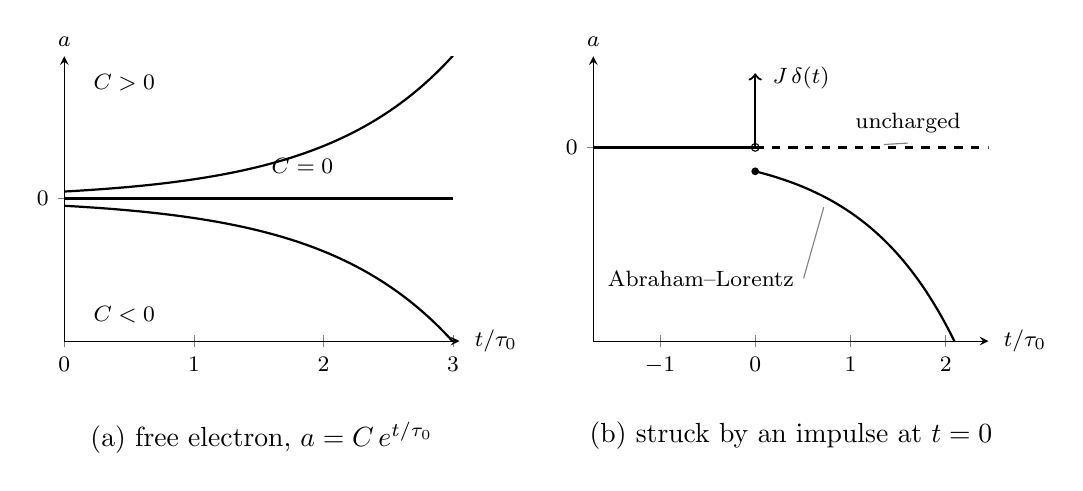
\begin{tikzpicture}

%% ---------------- panel (a): the free electron ----------------
\begin{axis}[
  name=free,
  width=6.6cm, height=5.2cm,
  xlabel={$t/\tau_0$}, ylabel={$a$},
  xmin=0, xmax=3.05, ymin=-3.2, ymax=3.2,
  axis lines=left,
  ytick={0}, yticklabels={$0$},
  xtick={0,1,2,3},
  every axis y label/.style={at={(ticklabel* cs:1.0)},anchor=south},
  every axis x label/.style={at={(ticklabel* cs:1.0)},anchor=west,
                             xshift=2pt},
  clip=true, samples=80, font=\footnotesize,
]
  \addplot[domain=0:3,thick] {0.16*exp(x)};
  \addplot[domain=0:3,thick] {-0.16*exp(x)};
  \addplot[domain=0:3,very thick] {0};
  \node[anchor=west,font=\footnotesize] at (axis cs:0.15,2.6)  {$C>0$};
  \node[anchor=west,font=\footnotesize] at (axis cs:0.15,-2.6) {$C<0$};
  \node[anchor=south east,font=\footnotesize] at (axis cs:2.15,0.35) {$C=0$};
\end{axis}
\node[anchor=north,align=center] at ([yshift=-9mm]free.south)
     {(a) free electron, $a=C\,e^{t/\tau_0}$};

%% ---------------- panel (b): struck by an impulse ----------------
\begin{axis}[
  name=imp,
  at={(free.east)}, anchor=west, xshift=1.7cm,
  width=6.6cm, height=5.2cm,
  xlabel={$t/\tau_0$}, ylabel={$a$},
  xmin=-1.7, xmax=2.45, ymin=-3.4, ymax=1.6,
  axis lines=left,
  ytick={0}, yticklabels={$0$},
  xtick={-1,0,1,2},
  every axis y label/.style={at={(ticklabel* cs:1.0)},anchor=south},
  every axis x label/.style={at={(ticklabel* cs:1.0)},anchor=west,
                             xshift=2pt},
  clip=true, samples=80, font=\footnotesize,
]
  %% before the blow: at rest
  \addplot[domain=-1.7:0,very thick] {0};
  %% uncharged particle: back to zero immediately
  \addplot[domain=0:2.45,very thick,dashed] {0};
  %% the impulse itself
  \draw[->,thick] (axis cs:0,0) -- (axis cs:0,1.3);
  \node[anchor=west,font=\footnotesize] at (axis cs:0.08,1.22) {$J\,\delta(t)$};
  %% Abraham-Lorentz: jumps the wrong way, then runs
  \addplot[domain=0:2.45,thick] {-0.42*exp(x)};
  \fill (axis cs:0,-0.42) circle (1.4pt);
  \draw (axis cs:0,0) circle (1.4pt);
  %% labels placed in the empty regions, with leaders
  \node[anchor=west,font=\footnotesize] (unch) at (axis cs:0.95,0.42)
       {uncharged};
  \draw[gray] (unch.south) -- (axis cs:1.35,0.05);
  \node[anchor=west,font=\footnotesize] (al) at (axis cs:-1.65,-2.3)
       {Abraham--Lorentz};
  \draw[gray] (al.east) -- (axis cs:0.72,-1.05);
\end{axis}
\node[anchor=north,align=center] at ([yshift=-9mm]imp.south)
     {(b) struck by an impulse at $t=0$};

\end{tikzpicture}
\caption{The two faces of the third-order term. \emph{(a)} A free electron
obeying Eq.~(\ref{eq:AL}) has $a = C\,e^{t/\tau_0}$. Every $C\ne0$ runs away;
the physical solution is the single value $C=0$, and nothing in the
initial-value problem selects it, since the equation is first order in $a$ and
admits any $a(0)$. \emph{(b)} An impulse delivered at $t=0$. An uncharged
particle takes the blow, jumps in velocity, and returns to zero acceleration:
the force is over and so is the acceleration. The electron does the opposite.
Its acceleration jumps to $\kappa = -J/m\tau_0$ and grows without bound long
after nothing is acting on it, and, since $\kappa$ carries the sign opposite to
$J$, it runs away against the blow that started it. The velocity, by contrast,
is continuous at $t=0$ here: it is the acceleration that jumps.
\label{fig:runaway}}
\end{figure}
.
%% Needs pgfplots, loaded in the main preamble.
%%
%% Panel (a) plots a = C exp(t/tau_0) for three values of C. Panel (b) plots
%% the impulse response of Eq. (AL): a = 0 before the blow and
%% a = kappa exp(t/tau_0) after it, with kappa = -J/(m tau_0). The sign is the
%% point of the panel and is not a drawing choice -- integrating
%% m a - m tau_0 adot = J delta(t) across t = 0 gives a jump of -J/(m tau_0),
%% so the runaway is directed against the impulse.

\begin{figure}[htb]
\centering
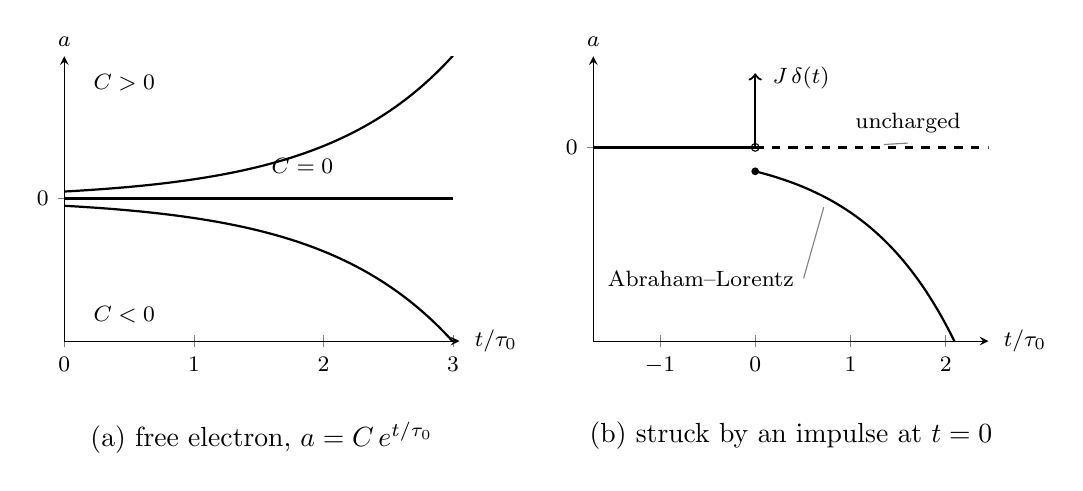
\begin{tikzpicture}

%% ---------------- panel (a): the free electron ----------------
\begin{axis}[
  name=free,
  width=6.6cm, height=5.2cm,
  xlabel={$t/\tau_0$}, ylabel={$a$},
  xmin=0, xmax=3.05, ymin=-3.2, ymax=3.2,
  axis lines=left,
  ytick={0}, yticklabels={$0$},
  xtick={0,1,2,3},
  every axis y label/.style={at={(ticklabel* cs:1.0)},anchor=south},
  every axis x label/.style={at={(ticklabel* cs:1.0)},anchor=west,
                             xshift=2pt},
  clip=true, samples=80, font=\footnotesize,
]
  \addplot[domain=0:3,thick] {0.16*exp(x)};
  \addplot[domain=0:3,thick] {-0.16*exp(x)};
  \addplot[domain=0:3,very thick] {0};
  \node[anchor=west,font=\footnotesize] at (axis cs:0.15,2.6)  {$C>0$};
  \node[anchor=west,font=\footnotesize] at (axis cs:0.15,-2.6) {$C<0$};
  \node[anchor=south east,font=\footnotesize] at (axis cs:2.15,0.35) {$C=0$};
\end{axis}
\node[anchor=north,align=center] at ([yshift=-9mm]free.south)
     {(a) free electron, $a=C\,e^{t/\tau_0}$};

%% ---------------- panel (b): struck by an impulse ----------------
\begin{axis}[
  name=imp,
  at={(free.east)}, anchor=west, xshift=1.7cm,
  width=6.6cm, height=5.2cm,
  xlabel={$t/\tau_0$}, ylabel={$a$},
  xmin=-1.7, xmax=2.45, ymin=-3.4, ymax=1.6,
  axis lines=left,
  ytick={0}, yticklabels={$0$},
  xtick={-1,0,1,2},
  every axis y label/.style={at={(ticklabel* cs:1.0)},anchor=south},
  every axis x label/.style={at={(ticklabel* cs:1.0)},anchor=west,
                             xshift=2pt},
  clip=true, samples=80, font=\footnotesize,
]
  %% before the blow: at rest
  \addplot[domain=-1.7:0,very thick] {0};
  %% uncharged particle: back to zero immediately
  \addplot[domain=0:2.45,very thick,dashed] {0};
  %% the impulse itself
  \draw[->,thick] (axis cs:0,0) -- (axis cs:0,1.3);
  \node[anchor=west,font=\footnotesize] at (axis cs:0.08,1.22) {$J\,\delta(t)$};
  %% Abraham-Lorentz: jumps the wrong way, then runs
  \addplot[domain=0:2.45,thick] {-0.42*exp(x)};
  \fill (axis cs:0,-0.42) circle (1.4pt);
  \draw (axis cs:0,0) circle (1.4pt);
  %% labels placed in the empty regions, with leaders
  \node[anchor=west,font=\footnotesize] (unch) at (axis cs:0.95,0.42)
       {uncharged};
  \draw[gray] (unch.south) -- (axis cs:1.35,0.05);
  \node[anchor=west,font=\footnotesize] (al) at (axis cs:-1.65,-2.3)
       {Abraham--Lorentz};
  \draw[gray] (al.east) -- (axis cs:0.72,-1.05);
\end{axis}
\node[anchor=north,align=center] at ([yshift=-9mm]imp.south)
     {(b) struck by an impulse at $t=0$};

\end{tikzpicture}
\caption{The two faces of the third-order term. \emph{(a)} A free electron
obeying Eq.~(\ref{eq:AL}) has $a = C\,e^{t/\tau_0}$. Every $C\ne0$ runs away;
the physical solution is the single value $C=0$, and nothing in the
initial-value problem selects it, since the equation is first order in $a$ and
admits any $a(0)$. \emph{(b)} An impulse delivered at $t=0$. An uncharged
particle takes the blow, jumps in velocity, and returns to zero acceleration:
the force is over and so is the acceleration. The electron does the opposite.
Its acceleration jumps to $\kappa = -J/m\tau_0$ and grows without bound long
after nothing is acting on it, and, since $\kappa$ carries the sign opposite to
$J$, it runs away against the blow that started it. The velocity, by contrast,
is continuous at $t=0$ here: it is the acceleration that jumps.
\label{fig:runaway}}
\end{figure}
